\chapter{Apprendimento democratizzato: Progettazione}\label{ch:chapter2}
In questo elaborato,studiamo un nuovo algoritmo di apprendimento distribuito che consiste in: raggruppamento gerarchico, generalizzazione gerarchica e meccanismi di apprendimento con un compito di apprendimento comune per tutti gli agenti di apprendimento.

\begin{itemize}

\item Meccanismo di raggruppamento gerarchico\\

Per costruire la struttura gerarchica del sistema Dem-AI con gruppi di apprendimento specializzati pertinenti, adottiamo l'algoritmo di clustering gerarchico agglomerativo ovvero l'implementazione del dendrogramma da scikit-learn, basato sulla somiglianza o non somiglianza di tutti gli agenti di apprendimento.
Il metodo del dendrogramma viene utilizzato per esaminare le relazioni di somiglianza tra gli individui ed è spesso utilizzato per l'analisi dei cluster in molti campi di ricerca. Durante l'implementazione, la topologia ad albero del dendrogramma viene costruita unendo le coppie di agenti o cluster che hanno la distanza minore tra loro, seguendo lo schema bottom-up. Di conseguenza, la distanza misurata è considerata come le differenze nelle caratteristiche degli agenti di apprendimento (ad esempio, parametri del modello locale o gradienti della funzione dell'obiettivo di apprendimento). Poiché otteniamo prestazioni simili implementando il clustering basato su parametri o gradienti del modello, in quanto segue presentiamo solo un meccanismo di clustering utilizzando i parametri del modello locale. \\
Dati i parametri del modello locale $\omega_n$ = ($\omega_{n,1}$,..., $\omega_{n,M}$) dell'agente di apprendimento \textsl{n}, dove \textsl{M} è il numero di parametri di apprendimento, la misura della distanza tra due agenti $\phi_{n,l}$ è derivata in base al modello euclideo distanza come $\phi_{n,l}$ =  ||$\omega_n$ - $\omega_l$|| 
Inoltre, consideriamo il metodo del collegamento medio per il calcolo della distanza tra un agente e un cluster utilizzando la distanza euclidea tra i parametri del modello dell'agente e i parametri del modello medio dei membri del cluster.
Di conseguenza, la struttura gerarchica ad albero è sotto forma di un albero binario con molti livelli. Richiederà quindi, costi computazionali e di archiviazione inutilmente elevati per mantenere i dati ed è un modo inefficiente per mantenere un gran numero di modelli generalizzati di basso livello per piccoli gruppi. Di conseguenza, manteniamo solo i K livelli superiori nella struttura ad albero e scartiamo la struttura di livello inferiore. Pertanto, al livello K più alto, il sistema potrebbe avere due grandi gruppi che hanno un gran numero di agenti di apprendimento.


\item Generalizzazione gerarchica e meccanismo di apprendimento\\

La struttura gerarchica di livello K emerge attraverso il clustering agglomerante. Di conseguenza, il sistema costruisce K livelli della generalizzazione, come in Figura. Pertanto, proponiamo problemi di apprendimento generalizzato gerarchico (HGLP) per costruire questi modelli generalizzati per gruppi specializzati in una forma ricorsiva, a partire dalla costruzione del modello globale $w^K$ al livello superiore \textsl{K} come segue. \\
Problema HGLP al livello K. \\\\
$\min_{W^{(K)}}L^{(K)}$ = $\sum_{i\in S_k} \frac{N_{g,i}^{(K-1)}}{N_g^{(K)}}L_i^{(K-1)}(w_i^{(K-1)}|D_i^{(K-1)})$ \hspace{2cm} (1)\\
s.t. $w^{(K)}=w_i^{(K-1)}, \forall i \in S_k$ \hspace{5cm} (2)\\
\\
Dove $W^{(K)}=(w^{(K)},w_1^{(K-1)},...,w_{|S_k|}^{(K-1)}), S_k$ è l'insieme dei sottogruppi del gruppo di livello superiore e $L_i^{(K-1)}$ è la funzione di perdita del sottogruppo \textsl{i} dato il suo set di dati collettivo $D_i$. La funzione obbiettivo è pesata su una frazione del numero di agenti totali $N_g^{()K-1}$ del sottogruppo \textsl{i} e $N_g^{(K)}$ agenti totali. Quindi i sottogruppi che hanno più agenti di apprendimento hanno un impatto superiore sul modello globale a livello \textbf{K}. I rigidi vincoli in (2) incoraggiano questi sottogruppi a condividere un modello di apprendimento comune. Per preservare le capacità di specializzazione di ciascun sottogruppo, questi vincoli (2) potrebbero essere allentati utilizzando termini prossimali aggiuntivi nell'obiettivo.
In questo modo, il problema incoraggia i modelli di apprendimento del sottogruppo ad avvicinarsi al modello globale ma non essendo necessariamente uguali. Pertanto, il problema rilassato HGLP' è definito come segue.
Problema HGLP' al livello K.\\\\
$\min_{W^{(K)}}\sum_{i\in S_k} \frac{N_{g,i}^{(K-1)}}{N_g^{(K)}}(L_i^{(K-1)}(w_i^{(K-1)}|D_i^{(K-1)}) +\frac{\mu_K}{2}||w^{(K)}-w_i^{(K-1)}||^2) $ \hspace{1cm} (3)\\
Dove $\mu_K$ denota il compromesso tra la perdita di apprendimento e il vincolo di generalizzazione che impone ai modelli di apprendimento di gruppo di essere vicini al modello globale $w^{(K)}$ . Poiché il set di dati è distribuito e disponibile solo presso gli agenti di apprendimento, il problema (3) al livello superiore \textbf{K} può essere risolto partendo prima dal problema dei suoi membri. Di conseguenza, la struttura gerarchica generalizzata è emersa naturalmente seguendo lo schema bottom-up in cui i modelli di apprendimento ai livelli inferiori vengono aggiornati prima di risolvere i problemi generalizzati di livello superiore del gruppo superiore. Nello specifico, il problema (3) può essere decentralizzato e risolto dal seguente problema di ciascun sottogruppo \textsl{i} al livello K - 1.
Problema HGLP per ogni gruppo \textsl{i} al livello K - 1.\\\\
$\min_{W^{(K-1)}}\sum_{j\in S_{i,K-1}} \frac{N_{g,j}^{(K-2)}}{N_g^{(K)}}(L_j^{(K-2)}(w_j^{(K-2)}|D_j^{(K-2)}) \\+\frac{\mu_{K-1}}{2}||w_j^{(K-2)}-w_i^{(K-1)}||^2)+ \frac{\mu_{K}N_{g,i}^{(K-1)}}{2N_g^{(K)}}||w^{(K)}-w_i^{(K-1)}||^2$\\\\
Dove $W^{(K-1)} = (w_i^{(K-1)},w_1^{(K-2)},...,w_{|S_{i,k-1}|}^{(K-2)})$ e facciamo una forma di approssimazione generale del problema generalizzato di apprendimento per il gruppo \textsl{i} a livello \textbf{K} dato il precedente modello generalizzato $w^{(k+1)}$ nel seguente modo.\\
Problema HGLP per ogni gruppo \textsl{i} al livello K.\\\\
$\min_{W^{(K)}}\sum_{j\in S_{i,K}} \frac{N_{g,j}^{(K-1)}}{N_g^{(K)}}(L_j^{(K-1)}(w_j^{(K-1)}|D_j^{(K-1)}) \\+\frac{\mu_{K}}{2}||w_j^{(K-1)}-w_i^{(K)}||^2)+ \frac{\mu_{K+1}N_{g,i}^{(K-1)}}{2N_g^{(K)}}||w^{(K+1)}-w_i^{(K)}||^2$ \hspace{1cm} (4)\\\\\\

Dove $W^{(K)} = (w_i^{(k)},w_1^{(k-1)},...,w_{|s_{i,k}|}^{(k-1)}),N_{g,i}^{(k)}$ è il numero di agenti di apprendimento del gruppo i, e $w^{(k+1)}$ è il modello di apprendimento del gruppo superiore al livello k + 1 a cui appartiene il gruppo i . Poiché esiste accoppiamento tra i livelli superiore e inferiore, e il set di dati di addestramento è decentralizzato, il problema di apprendimento (4) del gruppo i al livello k non può essere risolto direttamente.Quindi, analogamente a FL, la perdita di apprendimento del gruppo può essere distribuita tra i membri del gruppo [2]. Di conseguenza, l'obiettivo del problema di gruppo ha i restanti termini prossimali che costringono i modelli di apprendimento nei diversi livelli ad essere vicini l'uno all'altro. Pertanto, il modello di apprendimento è costruito con il modello del gruppo superiore a livello k + 1 e i membri del gruppo a livello k - 1 modellano risolvendo il seguente problema:\\
\\
$\min_{W}\sum_{j\in S_{i,K}} \frac{\mu_kN_{g,j}^{(K-1)}}{N_g^{(K)}}||w_j^{(k-1)}-w||^2+\frac{\mu_{K+1}N_{g,i}^{(k)}}{N_g^{(K)}}||w^{(K+1)}-w||^2$ \hspace{1cm} (5)\\\\\\
La forma chiusa della soluzione ottima del problema (5) può essere facilmente derivata impostando il gradiente a zero come segue:\\\\
$\sum_{j\in S_{i,K}}\mu_kN_{g,j}^{(k-1)}(w_j^{(k-1)}-w^*)=\mu_{k+1}N_{g,i}^{(k)}(w^*-w^{(k+1)})$\\
\\Pertanto, il modello di apprendimento del gruppo i può essere aggiornato come\\\\
$w_i^{(k)}=\alpha w^{(k+1)}+(1-\alpha)\sum_{j\in S_{(i,k)}}\frac{N_{g,j}^{(k)}}{N_{g,i}^{(k)}}w_j^{(k-1)}$ \hspace{1cm} (6)\\\\

Dove $\alpha=\mu_{(k+1)}/(\mu_k+\mu_{(k+1)})$. Il parametro di compromesso $\alpha$ può essere regolato successivamente negli esperimenti per controllare il contributo dei modelli di apprendimento dei membri del gruppo superiore e del gruppo. Data la soluzione in forma chiusa (6), l'accoppiamento tra diversi livelli
può essere approssimato suddividendo gli aggiornamenti del modello a ciascun livello tramite lo schema bottom-top e poi top bottom. In Fig. 3, mostriamo l'illustrazione degli aggiornamenti gerarchici proposti. In particolare, i gruppi e i membri inferiori vengono aggiornati prima dei gruppi superiori. E poi, i gruppi superiori aggiornati trasmettono i parametri ai loro membri del gruppo per completare un ciclo di aggiornamento.
Al livello più basso, ciascun agente di apprendimento \textsl{n} può effettivamente eseguire il processo di addestramento locale per adattare i propri dati privati al problema di apprendimento personalizzato utilizzando gli ultimi modelli gerarchici generalizzati come segue.\\
PLP al livello 0\\\\
$w_n^{(0)}=arg_{w\in W}min L_n^{(0)}(w|D_n^{(0)})+\frac{\mu}{2}||w-w_n^{(1)}||^2$\hspace{1cm} (7)\\\\
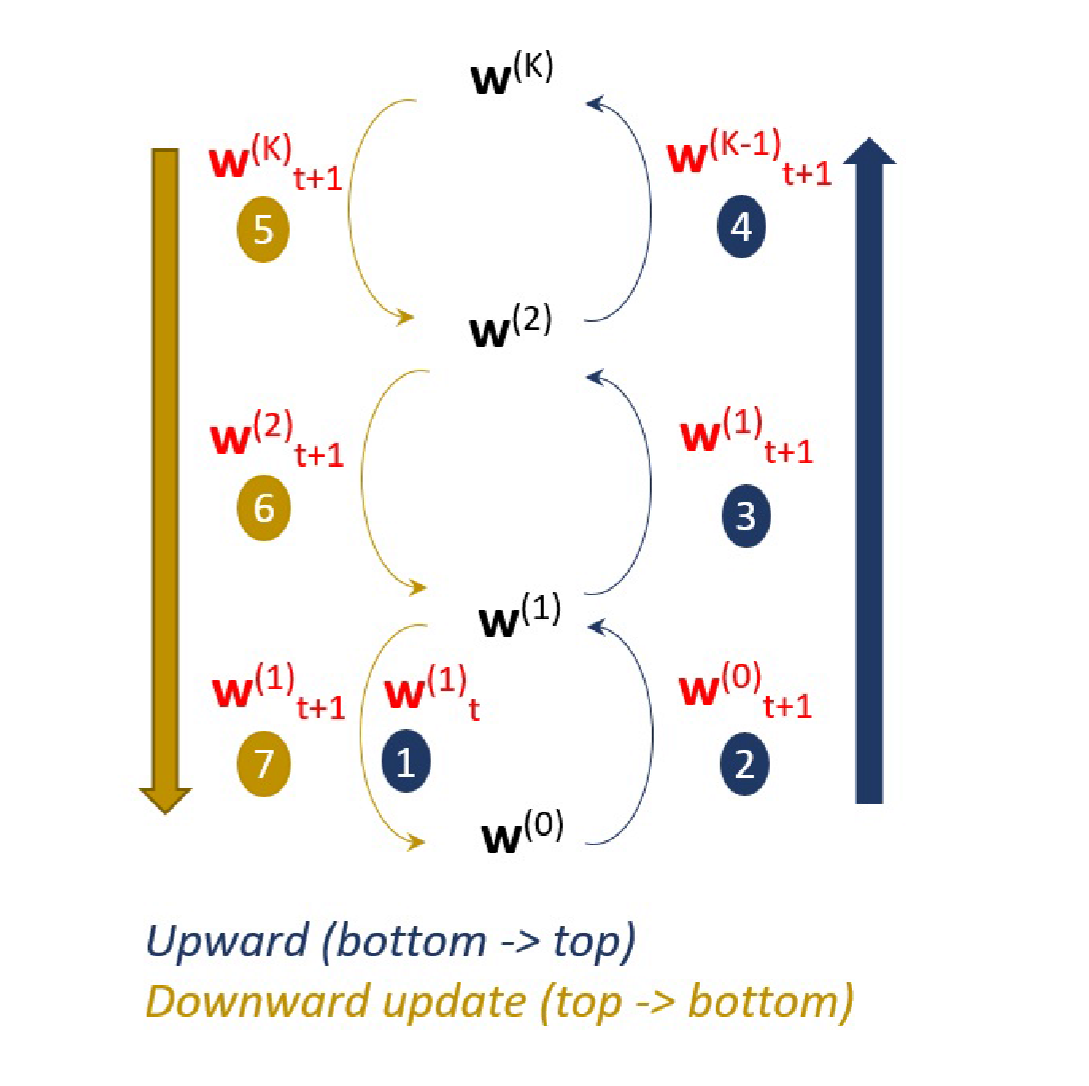
\includegraphics[scale=0.3]{BottomUPDOWN}\\
Dove $L_n^{(0)}$  è la funzione di perdita di apprendimento personalizzata per il compito di apprendimento dato il suo set di dati personalizzato $D_n^{(0)}$, $N_{(n,g)}^{(k)}$ è il numero di agenti di apprendimento del gruppo di livello-k a cui appartiene l'agente \textsl{n}.
Risolvendo il problema PLP, l'agente di apprendimento può aggiornare il proprio modello personalizzato $w_n^{(0)}$ appartenente al set di modelli di deep learning parametrizzato a W. In questo livello personalizzato, il numero di membri del gruppo è 1.

\item Algoritmo di apprendimento democratizzato.\\
Ispirati dagli algoritmi FedAvg e FedProx, adottiamo la
suddetta analisi ricorsiva e il meccanismo di clustering gerarchico per sviluppare un nuovo algoritmo di apprendimento democratizzato, chiamato DemLearn. I dettagli sono presentati di seguito. Ogni agente \textsl{n} usa il modello del gruppo superiore al livello 1 (cioè, $w_{(n,t)}^{(1)}$) come modello di apprendimento iniziale. Successivamente, l'agente risolve iterativamente il problema PLP nell'equazione (8) in base al metodo del gradiente.
Il modello client aggiornato verrà inviato al server centrale per eseguire il clustering gerarchico e l'aggiornamento dal livello 1 generalizzato al livello K. Dopo ogni giro globale $\tau$, la struttura gerarchica viene ricostruita in base ai cambiamenti nel modello di apprendimento personalizzato degli agenti. I modelli di apprendimento generalizzato dei gruppi vengono aggiornati, rispettivamente, in modalità bottom-top e top-bottom, seguendo (9) e (10) come approssimazione della soluzione in forma chiusa (6). Ciò consente ai sottogruppi di livello inferiore di contribuire con le proprie conoscenze all'aggiornamento del modello di gruppo. In cambio, ricevono (e incorporano) la migliore conoscenza generalizzata dai gruppi superiori che accresce la capacità di generalizzazione dei loro modelli di apprendimento locali. Inoltre, introduciamo un trucco di amplificazione nell'aggiornamento dal basso verso l'alto per i primi cinque round per accelerare la fase iniziale del processo di apprendimento. Di conseguenza, l'aggiornamento dai membri del gruppo [cioè, $w_{t+1}^{(k)}$ in (9)] viene moltiplicato con una costante di 1,15 nei primi cinque round.\\\\
\end{itemize}

\begin{algorithm}[H]
 \KwData{this text}
 \KwResult{how to write algorithm with \LaTeX2e }
 initialization\;
 \While{not at end of this document}{
  read current\;
  \eIf{understand}{
   go to next section\;
   current section becomes this one\;
   }{
   go back to the beginning of current section\;
  }
 }
 \caption{How to write algorithms}
\end{algorithm}


